% title: **Final Project**
% author:
% date: 2012-09-27
%
% f(x) = x^2
% \int f(x)

\documentclass[a4paper,12pt]{ctexart}


\usepackage{amsmath}
\usepackage{graphicx}


\usepackage{titlesec}
\titleformat{\section}{\large\bfseries}{\thesection}{.5em}{}

\begin{document}


% title
\title{Final Project}
\author{甘文迪 PB19030801}
\date{2022-6}

\maketitle
\pagestyle{empty}
\thispagestyle{empty}

考虑数值求解如下的优化问题

\begin{equation}
    \min_{u(x) \in C_0^1([0,1])}
    \int_{0}^{1} \left\{ \frac{1}{2}(u'(x))^2 + \frac{\alpha}{4}u^4(x) -f(x) u(x) \right\} \mathrm{d}x
\end{equation}


令 $h = \frac{1}{n},x_i = ih, i = 0, \ldots, n$。
记 $f_i = f(x_i)$,$u_i$ 为 $u(x_i)$ 的数值逼近,则 $u_0 = u_n = 0$。
用如下数值积分格式

\begin{equation}
    \min_{\{u_1, \ldots, u_{n-1}\}}
    \sum_{i=1}^n \frac{1}{2}\left(\frac{u_i - u_{i-1}}{h} \right)^2 h + \sum_{i=1}^{n-1} \left(\frac{\alpha}{4}u_i^4 - f_i u_i\right) h
\end{equation}

分别记 $u_h = \left(u_1, \ldots, u_{n-1}\right)^T$,$f_h = \left(f_1, \ldots, f_{n-1}\right)^T$。试回答如下问题


\section{当 $\alpha = 0$ 时,推导 $u_1, \ldots, u_{n-1}$ 满足的线性方程组 $A_h u_h = f_h$}

% grad T = 0
% pd T / pd u_i = 0

$$
\begin{aligned}
&T = \sum_{i=1}^n \frac{1}{2}\left(\frac{u_i - u_{i-1}}{h} \right)^2 h + \sum_{i=1}^{n-1} \left(\frac{\alpha}{4}u_i^4 - f_i u_i\right) h \\
&\frac{\partial T}{\partial u_k} = 0
\end{aligned}
$$

$$
\begin{aligned}\\
    \frac{\partial T}{\partial u_k} &= \frac{\partial}{\partial u_k}\left(
        \frac{1}{2}\left(\frac{u_k - u_{k-1}}{h} \right)^2 h +
        \frac{1}{2}\left(\frac{u_{k+1} - u_{k}}{h} \right)^2 h +
        \left(\frac{\alpha}{4}u_k^4 - f_k u_k\right) h \right) \\
    &=\frac{u_k - u_{k-1}}{h} -
        \frac{u_{k+1} - u_{k}}{h} +
        \left(\alpha u_k^3 - f_k\right) h =0 \\
    & 2u_k - u_{k+1} - u_{k-1} +  \left(\alpha u_k^3 - f_k\right) h^2 = 0
\end{aligned}
$$

当 $\alpha = 0$ 时,
$$
2u_k - u_{k+1} - u_{k-1} = f_k h^2
$$


$$
A_h = \begin{bmatrix}
    2 & -1 & 0 & 0 & \cdots & 0 & 0 \\
    -1 & 2 & -1 & 0 & \cdots & 0 & 0 \\
    0 & -1 & 2 & -1 & \cdots & 0 & 0 \\
    0 & 0 & -1 & 2 & \cdots & 0 & 0 \\
    \vdots & \vdots & \vdots & \vdots &    \ddots & \vdots & \vdots \\
    0 & 0 & 0 & 0 & \cdots & 2 & -1 \\
    0 & 0 & 0 & 0 & \cdots & -1 & 2
\end{bmatrix} / h^2
$$

$$
A_h u_h = f_h
$$



\section{当 $f(x) = \pi^2 \sin(\pi x)$,$n = 10, 20, 40, 80, 160$ 时,分别利用 Jacobi 和 Gauss-Seidel 方法求解 $A_h u_h = f_h$(迭代法的终止准则 $\varepsilon = 10^{-10}$),并比较 $u_h$ 与精确解 $u_e(x) = \sin(\pi x)$ 之间的误差 $e_h = ||u_h - u_e(x)||_2$,记录在一张表中}



当 $n = 10$ 时,用 Jacobi 方法求出的解为

$$
\begin{cases}
    u_1 = 0.3115711487  \\
    u_2 = 0.5926435426  \\
    u_3 = 0.8157038572  \\
    u_4 = 0.9589173951  \\
    u_5 = 1.0082654171  \\
    u_6 = 0.9589173951  \\
    u_7 = 0.8157038572  \\
    u_8 = 0.5926435426  \\
    u_9 = 0.3115711487  \\
\end{cases}
$$



\begin{table}[ht!]
\centering
\caption{Jacobi 和 Gauss-Seidel 方法求解 $A_h u_h = f_h$ 的误差 $e_h$}
% \label{tab:1.1}
\begin{tabular}{|c|c|c|}
\hline
$h$     &   Jacobi    &   Gauss-Seidel  \\    \hline
$\frac{1}{10}$      &   0.018482        &   0.018482    \\
$\frac{1}{20}$      &   0.006510        &   0.006510    \\
$\frac{1}{40}$      &   0.002300        &   0.002300    \\
$\frac{1}{80}$      &   0.000813        &   0.000813    \\
$\frac{1}{160}$     &   0.000287        &   0.000288    \\
\hline
\end{tabular}
\end{table}






\section{假设 (2) 中的 $u_h$ 对 (1) 的逼近误差满足 $e_h = \Theta(h^\beta)$,基于上表中的数据试利用最小二乘法找到 $\beta$}


作预处理,对两边求对数

$$
\begin{aligned}
e_h &= a h^\beta \\
\ln e_h &= \ln a + \beta \ln h \\
\end{aligned}
$$

计算 $\beta$,得到


% dot Jacobi beta = 1.501473
% dot Gauss Seidel beta = 1.501316

% itemize, space between lines is 0.5em
\begin{itemize}
    \setlength{\parskip}{0pt}
    \item Jacobi: $\beta = 1.5015$
    \item Gauss-Seidel: $\beta = 1.5013$
\end{itemize}

% show image/Jacobi.png
\begin{figure}[ht!]
\centering
\caption{Jacobi 方法求解的误差 $e_h$ 的拟合曲线}
% \label{fig:1.5}
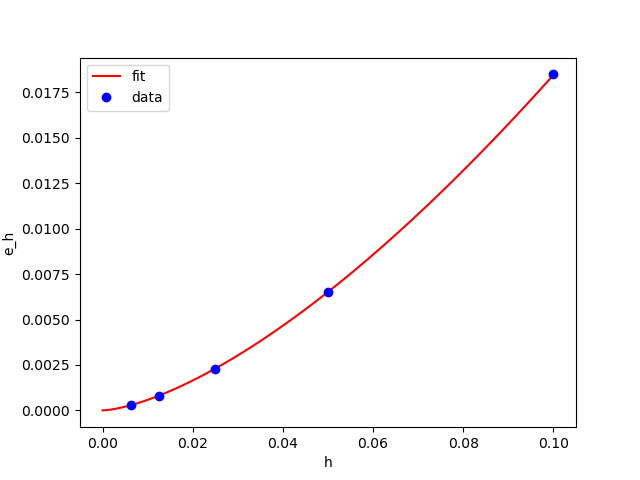
\includegraphics[width=0.6\textwidth]{image/Jacobi.png}
\end{figure}




\section{对 $n = 10, 20, 40, 80, 160$,分别记录 Jacobi 和 Gauss-Seidel 迭代法收敛所需要的迭代次数在同一张表中,从中你能得到什么结论?}

\begin{table}[ht!]
\centering
\caption{Jacobi 和 Gauss-Seidel 迭代法求解 $A_h u_h = f_h$ 的迭代次数}
% \label{tab:1.2}
\begin{tabular}{|c|c|c|}
\hline
n       &   Jacobi     &   Gauss-Seidel  \\    \hline
10      &   421        &   203    \\
20      &   1619       &   776    \\
40      &   6157       &   2939   \\
80      &   23296      &   11087  \\
160     &   87806      &   41652  \\
\hline
\end{tabular}
\end{table}

Gauss-Seidel 方法达到一定精度所需的迭代次数更少,大约是 Jacobi 方法的一半。
通过拟合,Jacobi 和 Gauss-Seidel 的迭代次数的增长阶大约是 1.91,接近二次。




\section{当 $\alpha = 1$,推导 $u_1, \ldots, u_{n-1}$ 满足的非线性方程组}


$$
2u_k - u_{k+1} - u_{k-1} +  \left(\alpha u_k^3 - f_k\right) h^2 = 0
$$


当 $\alpha = 1$ 时,

$$
2u_k - u_{k+1} - u_{k-1} + \left(u_k^3 - f_k\right) h^2 = 0
$$

$$
\begin{cases}
    2u_1 - u_2 - u_0 + (u_1^3 - f_1) h^2 = 0 \\
    2u_2 - u_3 - u_1 + (u_2^3 - f_2) h^2 = 0 \\
    \hspace{6.3em} \vdots \\
    2u_{n-1} - u_{n} - u_{n-2} + (u_{n-1}^3 - f_{n-1}) h^2 = 0
\end{cases}
$$


\section{当 $f(x) = \pi^2 \sin(\pi x) + \sin^3(\pi x)$,$n = 10, 20, 40, 80, 160$ 时,利用牛顿迭代法求解上一小题中的非线性方程组,并比较 $u_h$ 与精确解 $u_e(x) = \sin(\pi x)$ 之间的误差 $e_h = ||u_h - u_e(x)||_2$,记录在一张表中,并利用最小二乘法找出该情形下算法的收敛阶}



当 $n = 10$ 时,用牛顿迭代法求出的解为

$$
\begin{cases}
    u_1 = 0.31114144    \\
    u_2 = 0.59179025    \\
    u_3 = 0.81446878    \\
    u_4 = 0.95740830    \\
    u_5 = 1.00665582    \\
    u_6 = 0.95740830    \\
    u_7 = 0.81446878    \\
    u_8 = 0.59179025    \\
    u_9 = 0.31114144    \\
\end{cases}
$$

\begin{table}[ht!]
\centering
\caption{牛顿迭代法求解 $A_h u_h = f_h$ 的误差 $e_h$}
% \label{tab:1.3}
\begin{tabular}{|c|c|}
\hline
$n$     &   $e_h$  \\    \hline
10      &   0.015018    \\
20      &   0.005301    \\
40      &   0.001873    \\
80      &   0.000662    \\
160     &   0.000234    \\
\hline
\end{tabular}
\end{table}



用最小二乘法求出的收敛阶为 $\beta = 1.5007$

% show image/Newton.png
\begin{figure}[ht!]
\centering
\caption{牛顿迭代法求解的误差 $e_h$ 的拟合曲线}
% \label{fig:1.4}
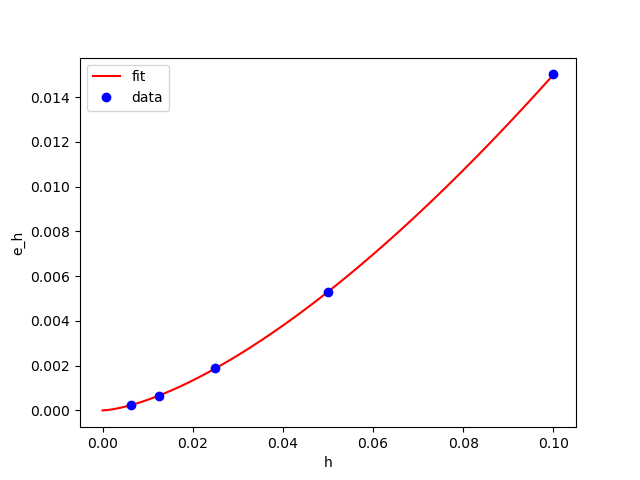
\includegraphics[width=0.6\textwidth]{image/Newton.png}
\end{figure}




\end{document}
